\subsection{Perturbation theory for the quartic oscillator}
\label{sec:253a-quartic-oscillator}

% YIN-SOURCE: id=PROPOSAL-B-U001; arguments=YIN253A-C02-A09; notes=253a:30; pdf=41; video=vk_RlYUKUyM:00:14:07.440-00:17:38.640; transcript=YIN253A-C02-T000485..YIN253A-C02-T000492; equations=YIN253A-C02-EQ013; class=SOURCE_COMPOSITE
We next consider the quartic oscillator. We set the oscillator frequency to
one and, until the ultraviolet discussion below, also set $\hbar=1$. The
coupling is normalized with a factor of $4!$:

% YIN-SOURCE: id=PROPOSAL-B-U002; arguments=YIN253A-C02-A09; notes=253a:30; pdf=41; video=vk_RlYUKUyM:00:14:40.139-00:16:52.519; transcript=YIN253A-C02-T000487..YIN253A-C02-T000491; equations=YIN253A-C02-EQ013; class=SOURCE_COMPOSITE
\begin{equation}
 \begin{aligned}
 H&=\frac{p^2}{2}+\frac{q^2}{2}+\frac{g}{4!}q^4,\\
 L&=\frac{1}{2}\dot q^{\,2}-\frac{q^2}{2}-\frac{g}{4!}q^4,\\
 L^E&=\frac{1}{2}(\partial_\tau q)^2+\frac{q^2}{2}+\frac{g}{4!}q^4.
 \end{aligned}
 \label{eq:253a-quartic-actions}
\end{equation}

% YIN-SOURCE: id=PROPOSAL-B-U003; arguments=YIN253A-C02-A09; notes=253a:30; pdf=41; video=vk_RlYUKUyM:00:15:37.800-00:20:46.039; transcript=YIN253A-C02-T000490..YIN253A-C02-T000502; equations=YIN253A-C02-EQ013; class=SOURCE_COMPOSITE
The spectral problem could be treated directly in the Hamiltonian formalism.
If you get confused, go back to your undergraduate quantum-mechanics textbook
and see how this system is studied there. Here we use the normalized Euclidean
two-point function, since its exponential falloffs contain the interacting
energy gaps:

% YIN-SOURCE: id=PROPOSAL-B-U004; arguments=YIN253A-C02-A09; notes=253a:30-31; pdf=41-42; video=vk_RlYUKUyM:00:17:05.400-00:22:55.640; transcript=YIN253A-C02-T000492..YIN253A-C02-T000507; equations=YIN253A-C02-EQ013; class=SOURCE_COMPOSITE
\begin{equation}
 \begin{aligned}
 G(\tau)&=\langle0|\widehat q(\tau)\widehat q(0)|0\rangle
 =\frac{1}{Z}\int[Dq]\,e^{-\int d\tau' L^E}\,q(\tau)q(0),
 \qquad \tau>0,\\
 Z&=\int[Dq]\,e^{-\int d\tau L^E}.
 \end{aligned}
 \label{eq:253a-quartic-correlator}
\end{equation}

% SOURCE-CONFLICT: Physical p. 42 explicitly warns that exchanging the functional integral with the power series in g is problematic. The proposal treats the result as an asymptotic perturbative expansion.
% YIN-SOURCE: id=PROPOSAL-B-U005; arguments=YIN253A-C02-A09; notes=253a:31; pdf=42; video=vk_RlYUKUyM:00:21:48.000-00:30:14.039; transcript=YIN253A-C02-T000506..YIN253A-C02-T000523; equations=YIN253A-C02-EQ013; class=SOURCE_COMPOSITE
Expanding the interaction exponential gives an asymptotic series whose
coefficients are Gaussian expectation values. With the subscript $0$ denoting
the harmonic oscillator,

% YIN-SOURCE: id=PROPOSAL-B-U006; arguments=YIN253A-C02-A09; notes=253a:31; pdf=42; video=vk_RlYUKUyM:00:21:48.000-00:30:14.039; transcript=YIN253A-C02-T000506..YIN253A-C02-T000523; equations=YIN253A-C02-EQ013; class=SOURCE_COMPOSITE
\begin{equation}
 \frac{Z_g}{Z_0}
 =\sum_{n=0}^{\infty}\frac{1}{n!}
 \left(-\frac{g}{4!}\right)^n
 \int d\tau_1\cdots d\tau_n\;
 \left\langle q^4(\tau_1)\cdots q^4(\tau_n)\right\rangle_0.
 \label{eq:253a-quartic-expansion}
\end{equation}

% YIN-SOURCE: id=PROPOSAL-B-U007; arguments=YIN253A-C02-A09; notes=253a:31-32; pdf=42-43; video=vk_RlYUKUyM:00:30:22.799-00:43:34.700; transcript=YIN253A-C02-T000524..YIN253A-C02-T000546; equations=YIN253A-C02-EQ014; class=SOURCE_COMPOSITE
At first order the four fields at the vertex admit three Wick pairings. At
second order the eight fields produce vacuum graphs with either one connected
component or several. Their algebraic contributions begin as

% SOURCE-CONFLICT: Physical p. 43 writes phi in the order-g^2 expectation while the surrounding model uses q. The proposal keeps q throughout the quartic-oscillator calculation.
% YIN-SOURCE: id=PROPOSAL-B-U008; arguments=YIN253A-C02-A09; notes=253a:31-32; pdf=42-43; video=vk_RlYUKUyM:00:31:26.460-00:43:34.700; transcript=YIN253A-C02-T000526..YIN253A-C02-T000546; equations=YIN253A-C02-EQ014; class=SOURCE_COMPOSITE
\begin{equation}
 \begin{aligned}
 -\frac{g}{4!}\int d\tau\,\langle q^4(\tau)\rangle_0
 &=-\frac{g}{8}\int d\tau\,\bigl(G_0(\tau,\tau)\bigr)^2,\\
 \left.\frac{Z_g}{Z_0}\right|_{g^2}
 &=\frac{1}{2}\left(-\frac{g}{4!}\right)^2
 \int d\tau_1\,d\tau_2\,
 \left\langle q^4(\tau_1)q^4(\tau_2)\right\rangle_0.
 \end{aligned}
 \label{eq:253a-first-vacuum-graphs}
\end{equation}

% YIN-SOURCE: id=PROPOSAL-B-U009; arguments=YIN253A-C02-A09,YIN253A-C02-A10; notes=253a:31-34; pdf=42-45; video=vk_RlYUKUyM:00:32:58.640-00:56:22.760; transcript=YIN253A-C02-T000528..YIN253A-C02-T000561; equations=YIN253A-C02-EQ014,YIN253A-C02-EQ015; class=SOURCE_COMPOSITE
\begin{figure}[H]
 \centering
 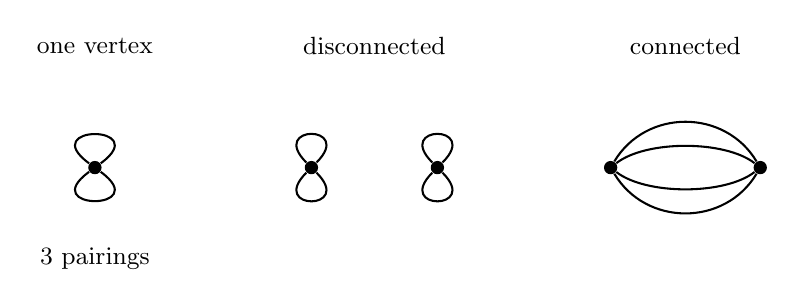
\begin{tikzpicture}[
   x=1cm,y=1cm,
   vertex/.style={circle,fill=black,inner sep=1.7pt},
   line/.style={line width=0.75pt},
   every node/.style={font=\small}
 ]
  \node at (-4.8,1.55) {one vertex};
  \node[vertex] (a) at (-4.8,0) {};
  \draw[line] (a) .. controls (-5.55,0.55) and (-4.05,0.55) .. (a);
  \draw[line] (a) .. controls (-5.55,-0.55) and (-4.05,-0.55) .. (a);
  \node at (-4.8,-1.15) {$3$ pairings};

  \node at (-1.25,1.55) {disconnected};
  \node[vertex] (b1) at (-2.05,0) {};
  \node[vertex] (b2) at (-0.45,0) {};
  \foreach \v in {b1,b2} {
    \draw[line] (\v) .. controls +(-0.55,0.55) and +(0.55,0.55) .. (\v);
    \draw[line] (\v) .. controls +(-0.55,-0.55) and +(0.55,-0.55) .. (\v);
  }

  \node at (2.7,1.55) {connected};
  \node[vertex] (c1) at (1.75,0) {};
  \node[vertex] (c2) at (3.65,0) {};
  \draw[line] (c1) .. controls (2.2,0.35) and (3.2,0.35) .. (c2);
  \draw[line] (c1) .. controls (2.2,0.75) and (3.2,0.75) .. (c2);
  \draw[line] (c1) .. controls (2.2,-0.35) and (3.2,-0.35) .. (c2);
  \draw[line] (c1) .. controls (2.2,-0.75) and (3.2,-0.75) .. (c2);
 \end{tikzpicture}
 \caption{The first vacuum Wick topologies. A quartic vertex carries
 $-g/4!$, and every line denotes a free propagator $G_0$.}
 \label{fig:253a-vacuum-topologies}
\end{figure}

% YIN-SOURCE: id=PROPOSAL-B-U010; arguments=YIN253A-C02-A09; notes=253a:31-32; pdf=42-43; video=vk_RlYUKUyM:00:23:45.720-00:39:48.680; transcript=YIN253A-C02-T000510..YIN253A-C02-T000539; equations=YIN253A-C02-EQ013,YIN253A-C02-EQ014; class=SOURCE_COMPOSITE
The perturbation series has zero radius of convergence. Its coefficients
still give useful finite-order approximations at small $g$. In fact, as often
occurs here, this asymptotic behavior is a feature of the expansion.

\subsection{Connected vacuum graphs and the ground-state energy}
\label{sec:253a-connected-vacuum-graphs}

% YIN-SOURCE: id=PROPOSAL-B-U011; arguments=YIN253A-C02-A10; notes=253a:33-34; pdf=44-45; video=vk_RlYUKUyM:00:45:10.920-00:55:12.720; transcript=YIN253A-C02-T000549..YIN253A-C02-T000560; equations=YIN253A-C02-EQ014,YIN253A-C02-EQ015; class=SOURCE_COMPOSITE
The vacuum graphs have a simple organization. Suppose a graph at order $g^n$
has $m_\ell$ connected components containing $\ell$ vertices. Then

% YIN-SOURCE: id=PROPOSAL-B-U012; arguments=YIN253A-C02-A10; notes=253a:33; pdf=44; video=vk_RlYUKUyM:00:47:01.500-00:51:16.260; transcript=YIN253A-C02-T000552..YIN253A-C02-T000556; equations=YIN253A-C02-EQ014,YIN253A-C02-EQ015; class=SOURCE_COMPOSITE
\begin{equation}
 \sum_{\ell\geq1}m_\ell=K,
 \qquad
 \sum_{\ell\geq1}\ell m_\ell=n,
 \qquad
 N(\{m_\ell\})=
 \frac{n!}{\displaystyle\prod_{\ell\geq1}(\ell!)^{m_\ell}m_\ell!}.
 \label{eq:253a-component-partition}
\end{equation}

% YIN-SOURCE: id=PROPOSAL-B-U013; arguments=YIN253A-C02-A10; notes=253a:34; pdf=45; video=vk_RlYUKUyM:00:53:01.280-00:55:12.720; transcript=YIN253A-C02-T000559..YIN253A-C02-T000560; equations=YIN253A-C02-EQ015; class=SOURCE_COMPOSITE
Let $G^{(\ell)}$ denote the complete contribution from connected Wick
contractions of $\ell$ vertices, including the vertex factors and integrations.
For a fixed component pattern, the factor $1/n!$ from the exponential combines
with the grouping count to give

% YIN-SOURCE: id=PROPOSAL-B-U014; arguments=YIN253A-C02-A10; notes=253a:33-34; pdf=44-45; video=vk_RlYUKUyM:00:53:01.280-00:55:12.720; transcript=YIN253A-C02-T000559..YIN253A-C02-T000560; equations=YIN253A-C02-EQ015; class=SOURCE_COMPOSITE
\begin{equation}
 \frac{1}{n!}N(\{m_\ell\})
 \prod_{\ell\geq1}\bigl(G^{(\ell)}\bigr)^{m_\ell}
 =\prod_{\ell\geq1}\frac{1}{m_\ell!}
 \left(\frac{G^{(\ell)}}{\ell!}\right)^{m_\ell}.
 \label{eq:253a-component-weight}
\end{equation}

% YIN-SOURCE: id=PROPOSAL-B-U015; arguments=YIN253A-C02-A10; notes=253a:34; pdf=45; video=vk_RlYUKUyM:00:55:10.559-00:59:44.359; transcript=YIN253A-C02-T000561..YIN253A-C02-T000565; equations=YIN253A-C02-EQ015; class=SOURCE_COMPOSITE
The sums over the nonnegative integers $m_\ell$ are independent. Each one is
the Taylor series of an exponential, and consequently

% YIN-SOURCE: id=PROPOSAL-B-U016; arguments=YIN253A-C02-A10; notes=253a:34; pdf=45; video=vk_RlYUKUyM:00:57:03.660-00:59:44.359; transcript=YIN253A-C02-T000563..YIN253A-C02-T000565; equations=YIN253A-C02-EQ015; class=SOURCE_COMPOSITE
\begin{equation}
 \frac{Z_g}{Z_0}
 =\sum_{\{m_\ell\}}\prod_{\ell\geq1}\frac{1}{m_\ell!}
 \left(\frac{G^{(\ell)}}{\ell!}\right)^{m_\ell}
 =\exp\left(\sum_{\ell\geq1}\frac{G^{(\ell)}}{\ell!}\right).
 \label{eq:253a-connected-exponentiation}
\end{equation}

% YIN-SOURCE: id=PROPOSAL-B-U017; arguments=YIN253A-C02-A10; notes=253a:34; pdf=45; video=vk_RlYUKUyM:00:58:21.180-00:59:44.359; transcript=YIN253A-C02-T000564..YIN253A-C02-T000565; equations=YIN253A-C02-EQ015; class=SOURCE_COMPOSITE
Thus $\log(Z_g/Z_0)$ retains the connected vacuum graphs. The disconnected
ones are generated with their factorials when the exponential is expanded.
This follows from the expansion itself, so every disconnected graph need not
be counted afresh.

% YIN-SOURCE: id=PROPOSAL-B-U018; arguments=YIN253A-C02-A10; notes=253a:34; pdf=45; video=vk_RlYUKUyM:00:55:10.559-00:56:22.760; transcript=YIN253A-C02-T000561..YIN253A-C02-T000561; equations=YIN253A-C02-EQ015; class=SOURCE_COMPOSITE
For example, one connected three-vertex contribution is

% YIN-SOURCE: id=PROPOSAL-B-U019; arguments=YIN253A-C02-A10; notes=253a:34; pdf=45; video=vk_RlYUKUyM:00:55:10.559-00:56:22.760; transcript=YIN253A-C02-T000561..YIN253A-C02-T000561; equations=YIN253A-C02-EQ015; class=SOURCE_COMPOSITE
\begin{equation}
 \frac{1}{3!}\left(-\frac{g}{4!}\right)^3
 \int d\tau_1\,d\tau_2\,d\tau_3\;
 G_0(\tau_1,\tau_2)^2G_0(\tau_2,\tau_3)^2
 G_0(\tau_3,\tau_1)^2.
 \label{eq:253a-three-vertex-connected}
\end{equation}

% YIN-SOURCE: id=PROPOSAL-B-U020; arguments=YIN253A-C02-A10; notes=253a:34-36; pdf=45-47; video=vk_RlYUKUyM:00:55:10.559-01:16:44.179; transcript=YIN253A-C02-T000561..YIN253A-C02-T000593; equations=YIN253A-C02-EQ015,YIN253A-C02-EQ016; class=SOURCE_COMPOSITE
Translation invariance leaves one unrestricted common Euclidean time in a
connected vacuum graph. The remaining relative-time integrals converge
because the propagators decay exponentially. By definition, the connected
contribution therefore has one extensive factor proportional to $T$.

% YIN-SOURCE: id=PROPOSAL-B-U021; arguments=YIN253A-C02-A10; notes=253a:35-36; pdf=46-47; video=vk_RlYUKUyM:01:07:07.799-01:12:01.640; transcript=YIN253A-C02-T000580..YIN253A-C02-T000587; equations=YIN253A-C02-EQ016; class=SOURCE_COMPOSITE
On an interval of length $T$, the Euclidean path integral is a matrix element
of $e^{-HT}$. A unique ground state dominates at large $T$, provided the
endpoint states have nonzero ground-state overlap. Hence

% YIN-SOURCE: id=PROPOSAL-B-U022; arguments=YIN253A-C02-A10; notes=253a:35-36; pdf=46-47; video=vk_RlYUKUyM:01:07:34.799-01:12:01.640; transcript=YIN253A-C02-T000581..YIN253A-C02-T000587; equations=YIN253A-C02-EQ016; class=SOURCE_COMPOSITE
\begin{equation}
 Z=\langle q_f|e^{-HT}|q_i\rangle,
 \qquad
 \log Z=-E_0T+O(1),
 \qquad
 E_0=-\lim_{T\to\infty}\frac{1}{T}\log Z.
 \label{eq:253a-vacuum-energy}
\end{equation}

% SOURCE-CONFLICT: Physical p. 47 writes G in the first free-propagator reminder and G_0 in the coincident reminder. The proposal uses G_0 for both free quantities.
% YIN-SOURCE: id=PROPOSAL-B-U023; arguments=YIN253A-C02-A10; notes=253a:36-37; pdf=47-48; video=vk_RlYUKUyM:01:12:02.960-01:17:16.280; transcript=YIN253A-C02-T000588..YIN253A-C02-T000594; equations=YIN253A-C02-EQ016; class=SOURCE_COMPOSITE
At first order, $G_0(\tau,\tau)=1/(2\omega)$ gives the energy shift. In the
local convention $\omega=1$, the same result follows from ordinary Hamiltonian
perturbation theory:

% YIN-SOURCE: id=PROPOSAL-B-U024; arguments=YIN253A-C02-A10; notes=253a:36-37; pdf=47-48; video=vk_RlYUKUyM:01:12:02.960-01:15:44.219; transcript=YIN253A-C02-T000588..YIN253A-C02-T000592; equations=YIN253A-C02-EQ016; class=SOURCE_COMPOSITE
\begin{equation}
 \begin{aligned}
 \Delta E_0&=\frac{g}{8}\left(\frac{1}{2\omega}\right)^2+O(g^2),\\
 \left.\Delta E_0\right|_{\omega=1}
 &=\langle\psi_0|H_1|\psi_0\rangle
 =\frac{g}{4!}\langle\widehat q^{\,4}\rangle_0
 =\frac{g}{4!}\frac{3}{4}=\frac{g}{32}.
 \end{aligned}
 \label{eq:253a-first-vacuum-energy-shift}
\end{equation}

\subsection{The normalized two-point function and self-energy}
\label{sec:253a-self-energy}

% YIN-SOURCE: id=PROPOSAL-B-U025; arguments=YIN253A-C02-A11; notes=253a:38-39; pdf=49-50; video=3VG2kDHso08:00:01:10.080-00:14:08.540; transcript=YIN253A-C02-T000608..YIN253A-C02-T000630; equations=YIN253A-C02-EQ017; class=SOURCE_COMPOSITE
We return to the normalized correlator and expand its numerator. Every Wick
graph factors into a component containing the two external insertions and a
collection of vacuum components. The sum over those vacuum components is
precisely $Z$, so it cancels the factor $1/Z$.

% YIN-SOURCE: id=PROPOSAL-B-U026; arguments=YIN253A-C02-A11; notes=253a:38-39; pdf=49-50; video=3VG2kDHso08:00:05:42.900-00:14:08.540; transcript=YIN253A-C02-T000616..YIN253A-C02-T000630; equations=YIN253A-C02-EQ017; class=SOURCE_COMPOSITE
\begin{figure}[H]
 \centering
 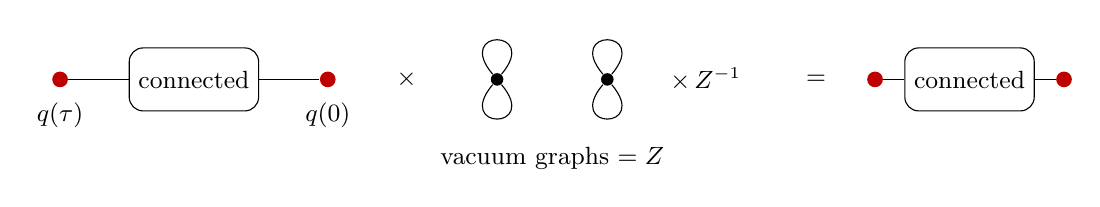
\begin{tikzpicture}[
   x=1cm,y=1cm,
   ext/.style={circle,fill=red!75!black,inner sep=2pt},
   vertex/.style={circle,fill=black,inner sep=1.6pt},
  blob/.style={draw,rounded corners=5pt,minimum width=1.55cm,minimum height=0.8cm},
   every node/.style={font=\small}
 ]
  \node[ext] (x1) at (-5.2,0) {};
  \node[blob] (conn) at (-3.5,0) {connected};
  \node[ext] (x2) at (-1.8,0) {};
  \draw (x1)--(conn)--(x2);
  \node at (-5.2,-0.45) {$q(\tau)$};
  \node at (-1.8,-0.45) {$q(0)$};
  \node at (-0.8,0) {$\times$};
  \node[vertex] (v1) at (0.35,0) {};
  \node[vertex] (v2) at (1.75,0) {};
  \draw (v1) .. controls (-0.2,0.65) and (0.9,0.65) .. (v1);
  \draw (v1) .. controls (-0.2,-0.65) and (0.9,-0.65) .. (v1);
  \draw (v2) .. controls (1.2,0.65) and (2.3,0.65) .. (v2);
  \draw (v2) .. controls (1.2,-0.65) and (2.3,-0.65) .. (v2);
  \node at (1.05,-1.0) {vacuum graphs $=Z$};
  \node at (3.0,0) {$\times\,Z^{-1}$};
  \node at (4.4,0) {$=$};
  \node[ext] (y1) at (5.15,0) {};
  \node[blob] (c2) at (6.35,0) {connected};
  \node[ext] (y2) at (7.55,0) {};
  \draw (y1)--(c2)--(y2);
 \end{tikzpicture}
 \caption{Vacuum components in the two-point numerator cancel against its
 normalization. The surviving graph connects the two external insertions.}
 \label{fig:253a-vacuum-cancellation}
\end{figure}

% YIN-SOURCE: id=PROPOSAL-B-U027; arguments=YIN253A-C02-A11; notes=253a:39; pdf=50; video=3VG2kDHso08:00:14:43.199-00:24:05.400; transcript=YIN253A-C02-T000632..YIN253A-C02-T000646; equations=YIN253A-C02-EQ017; class=SOURCE_COMPOSITE
The graph is an easy way to organize the possible contractions, while the
combinatorial factors still have to be calculated. The free external line is
the harmonic-oscillator Green function,

% YIN-SOURCE: id=PROPOSAL-B-U028; arguments=YIN253A-C02-A11; notes=253a:39; pdf=50; video=3VG2kDHso08:00:21:25.380-00:24:05.400; transcript=YIN253A-C02-T000643..YIN253A-C02-T000646; equations=YIN253A-C02-EQ017; class=SOURCE_COMPOSITE
\begin{equation}
 \begin{aligned}
 \langle q(\tau)q(0)\rangle
 &=\begin{cases}
 \langle0|\widehat q(\tau)\widehat q(0)|0\rangle,&\tau\geq0,\\[2pt]
 \langle0|\widehat q(0)\widehat q(\tau)|0\rangle,&\tau<0,
 \end{cases}\\
 G_0(\tau)&=\frac{1}{2}e^{-|\tau|}
 =\int\frac{dk}{2\pi}\,\widetilde G_0(k)e^{ik\tau},
 \qquad
 \widetilde G_0(k)=\frac{1}{k^2+1}.
 \end{aligned}
 \label{eq:253a-free-euclidean-propagator}
\end{equation}

% YIN-SOURCE: id=PROPOSAL-B-U029; arguments=YIN253A-C02-A11,YIN253A-C02-A12; notes=253a:40; pdf=51; video=3VG2kDHso08:00:24:01.260-00:34:20.599; transcript=YIN253A-C02-T000647..YIN253A-C02-T000663; equations=YIN253A-C02-EQ018; class=SOURCE_COMPOSITE
For the one-vertex correction, an external $q$ can be contracted with any of
the four fields at the vertex. The second external $q$ then has three choices.
Four times three. The remaining fields have to contract with one another, and
that is it. Together with $-g/4!$, the count gives $-g/2$:

% YIN-SOURCE: id=PROPOSAL-B-U030; arguments=YIN253A-C02-A11,YIN253A-C02-A12; notes=253a:40; pdf=51; video=3VG2kDHso08:00:25:16.620-00:33:47.539; transcript=YIN253A-C02-T000649..YIN253A-C02-T000662; equations=YIN253A-C02-EQ018; class=SOURCE_COMPOSITE
\begin{equation}
 \begin{aligned}
 G^{(1)}(\tau)
 &=-\frac{g}{2}\int d\tau'\,
 G_0(\tau-\tau')G_0(\tau')G_0(0)\\
 &=-\frac{g}{2}\cdot\frac{1}{2}
 \int\frac{dk}{2\pi}\frac{e^{ik\tau}}{(k^2+1)^2}.
 \end{aligned}
 \label{eq:253a-tadpole-correction}
\end{equation}

% YIN-SOURCE: id=PROPOSAL-B-U031; arguments=YIN253A-C02-A12; notes=253a:40-41; pdf=51-52; video=3VG2kDHso08:00:27:46.559-00:43:46.339; transcript=YIN253A-C02-T000653..YIN253A-C02-T000681; equations=YIN253A-C02-EQ018; class=SOURCE_COMPOSITE
It is important to get this counting correct. Fourier space provides a useful
check: assign an orientation to every line, impose wave-number conservation at
each vertex, and integrate every independent loop variable. If a rule becomes
confusing, go back to the formula that defines the graph.

% YIN-SOURCE: id=PROPOSAL-B-U032; arguments=YIN253A-C02-A12; notes=253a:41; pdf=52; video=3VG2kDHso08:00:39:57.900-00:50:36.480; transcript=YIN253A-C02-T000675..YIN253A-C02-T000695; equations=YIN253A-C02-EQ018; class=SOURCE_COMPOSITE
What does 1PI stand for? A two-point graph is one-particle irreducible when
cutting any single internal propagator leaves the two external sides connected.
The self-energy $\Sigma(k)$ is the sum of these 1PI graphs after their external
free propagators have been amputated.

% YIN-SOURCE: id=PROPOSAL-B-U033; arguments=YIN253A-C02-A12; notes=253a:41; pdf=52; video=3VG2kDHso08:00:40:36.920-00:50:36.480; transcript=YIN253A-C02-T000676..YIN253A-C02-T000695; equations=YIN253A-C02-EQ018; class=SOURCE_COMPOSITE
\begin{figure}[H]
 \centering
 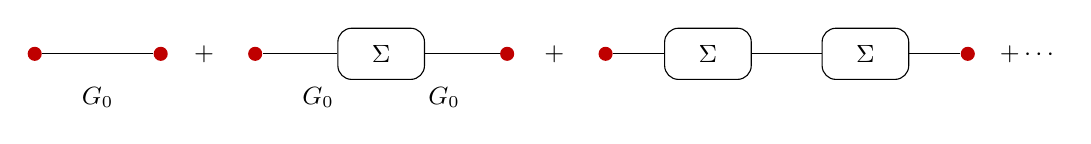
\begin{tikzpicture}[
   x=1cm,y=1cm,
   ext/.style={circle,fill=red!75!black,inner sep=1.8pt},
  insertion/.style={draw,rounded corners=5pt,minimum width=1.1cm,minimum height=0.65cm},
   every node/.style={font=\small}
 ]
  \node[ext] (a0) at (-6.4,0) {};
  \node[ext] (a1) at (-4.8,0) {};
  \draw (a0)--(a1);
  \node at (-5.6,-0.55) {$G_0$};
  \node at (-4.25,0) {$+$};

  \node[ext] (b0) at (-3.6,0) {};
  \node[insertion] (s1) at (-2.0,0) {$\Sigma$};
  \node[ext] (b1) at (-0.4,0) {};
  \draw (b0)--(s1)--(b1);
  \node at (-2.8,-0.55) {$G_0$};
  \node at (-1.2,-0.55) {$G_0$};
  \node at (0.2,0) {$+$};

  \node[ext] (c0) at (0.85,0) {};
  \node[insertion] (s2) at (2.15,0) {$\Sigma$};
  \node[insertion] (s3) at (4.15,0) {$\Sigma$};
  \node[ext] (c1) at (5.45,0) {};
  \draw (c0)--(s2)--(s3)--(c1);
  \node at (6.2,0) {$+\cdots$};
 \end{tikzpicture}
 \caption{The full connected two-point function as a chain of amputated 1PI
 insertions separated by free propagators.}
 \label{fig:253a-1pi-chain}
\end{figure}

% YIN-SOURCE: id=PROPOSAL-B-U034; arguments=YIN253A-C02-A12; notes=253a:41; pdf=52; video=3VG2kDHso08:00:45:02.040-00:52:48.900; transcript=YIN253A-C02-T000685..YIN253A-C02-T000698; equations=YIN253A-C02-EQ018; class=SOURCE_COMPOSITE
Repeated insertions form a geometric series. The external $G_0$ factors remain
outside the definition of $\Sigma$, giving

% YIN-SOURCE: id=PROPOSAL-B-U035; arguments=YIN253A-C02-A12; notes=253a:41; pdf=52; video=3VG2kDHso08:00:48:55.859-00:52:48.900; transcript=YIN253A-C02-T000693..YIN253A-C02-T000698; equations=YIN253A-C02-EQ018; class=SOURCE_COMPOSITE
\begin{equation}
 \begin{aligned}
 G(\tau)
 &=\int\frac{dk}{2\pi}e^{ik\tau}\widetilde G_0(k)
 \sum_{n=0}^{\infty}
 \bigl(\widetilde G_0(k)\Sigma(k)\bigr)^n\\
 &=\int\frac{dk}{2\pi}\frac{e^{ik\tau}}{k^2+1-\Sigma(k)},\\
 \Sigma(k)&=-\frac{g}{4}
 +\frac{g^2}{8}\left(\frac{1}{4}+\frac{1}{k^2+9}\right)+O(g^3).
 \end{aligned}
 \label{eq:253a-self-energy-resummation}
\end{equation}

\subsection{Poles and the interacting energy gap}
\label{sec:253a-dressed-poles}

% YIN-SOURCE: id=PROPOSAL-B-U036; arguments=YIN253A-C02-A13; notes=253a:42-43; pdf=53-54; video=3VG2kDHso08:00:56:20.780-01:02:56.540; transcript=YIN253A-C02-T000704..YIN253A-C02-T000715; equations=YIN253A-C02-EQ019; class=SOURCE_COMPOSITE
How would one read the energy spectrum from this Fourier representation? At
first look, this is pretty weird: the Fourier integral contains $e^{ik\tau}$,
while the spectral representation contains decaying real exponentials. The two
forms of the same function are

% YIN-SOURCE: id=PROPOSAL-B-U037; arguments=YIN253A-C02-A13; notes=253a:42; pdf=53; video=3VG2kDHso08:00:56:20.780-01:02:56.540; transcript=YIN253A-C02-T000704..YIN253A-C02-T000715; equations=YIN253A-C02-EQ019; class=SOURCE_COMPOSITE
\begin{equation}
 \begin{aligned}
 G(\tau)&=\int\frac{dk}{2\pi}\,\widetilde G(k)e^{ik\tau},\\
 \widetilde G(k)&=
 \frac{1}{k^2+1+\frac{g}{4}
 -\frac{g^2}{8}\left(\frac{1}{4}+\frac{1}{k^2+9}\right)+O(g^3)},\\
 G(\tau)&=\sum_n
 \left|\langle n|\widehat q(0)|0\rangle\right|^2
 e^{-(\bar E_n-\bar E_0)\tau},
 \qquad \tau>0.
 \end{aligned}
 \label{eq:253a-dressed-and-spectral}
\end{equation}

% SOURCE-CONFLICT: The pole sketch on physical p. 53 has a labelled real axis, no Im k label, two labelled upper poles, and unlabelled lower poles. The proposal draws only the upper-half-plane data used for positive tau.
% YIN-SOURCE: id=PROPOSAL-B-U038; arguments=YIN253A-C02-A13; notes=253a:42-43; pdf=53-54; video=3VG2kDHso08:01:02:26.040-01:06:29.640; transcript=YIN253A-C02-T000714..YIN253A-C02-T000722; equations=YIN253A-C02-EQ019; class=SOURCE_COMPOSITE
\begin{figure}[H]
 \centering
 \begin{tikzpicture}[x=1cm,y=1cm,>=Latex,every node/.style={font=\small}]
  \draw[->] (-4,0)--(4.3,0) node[right] {$\operatorname{Re}k$};
  \draw[line width=0.9pt,blue!65!black,->]
    (-3.6,0) arc (180:12:3.6);
  \node[red!75!black] at (0,1.0) {$\times$};
  \node[anchor=west] at (0.18,1.0) {$i\omega_1$};
  \node[red!75!black] at (0,2.05) {$\times$};
  \node[anchor=west] at (0.18,2.05) {$i\omega_2$};
  \node at (0,2.75) {$\vdots$};
 \end{tikzpicture}
 \caption{For $\tau>0$, the contour closes in the upper half-plane. Each pole
 at $k=i\omega_n$ supplies a decaying exponential.}
 \label{fig:253a-dressed-poles}
\end{figure}

% YIN-SOURCE: id=PROPOSAL-B-U039; arguments=YIN253A-C02-A13; notes=253a:43; pdf=54; video=3VG2kDHso08:01:03:01.740-01:10:03.440; transcript=YIN253A-C02-T000716..YIN253A-C02-T000727; equations=YIN253A-C02-EQ019; class=SOURCE_COMPOSITE
For positive $\tau$, the factor $e^{ik\tau}$ suppresses the large upper
semicircle. The residue theorem then turns each pole into a spectral
exponential:

% YIN-SOURCE: id=PROPOSAL-B-U040; arguments=YIN253A-C02-A13; notes=253a:43; pdf=54; video=3VG2kDHso08:01:03:01.740-01:10:03.440; transcript=YIN253A-C02-T000716..YIN253A-C02-T000727; equations=YIN253A-C02-EQ019; class=SOURCE_COMPOSITE
\begin{equation}
 \int\frac{dk}{2\pi}\,\widetilde G(k)e^{ik\tau}
 =i\sum_n e^{-\omega_n\tau}
 \underset{k\to i\omega_n}{\operatorname{Res}}\widetilde G(k),
 \qquad
 \omega_n=\bar E_n-\bar E_0.
 \label{eq:253a-pole-spectral-map}
\end{equation}

% SOURCE-CONFLICT: Physical p. 53 ends the denominator with O(g^3), while p. 54 repeats it with four continuation dots and a comma. The proposal uses the reconciled O(g^3) remainder.
% YIN-SOURCE: id=PROPOSAL-B-U041; arguments=YIN253A-C02-A13; notes=253a:43; pdf=54; video=3VG2kDHso08:01:08:42.739-01:12:06.239; transcript=YIN253A-C02-T000725..YIN253A-C02-T000730; equations=YIN253A-C02-EQ019; class=SOURCE_COMPOSITE
The free pole at $k=i$ shifts when the quartic coupling is turned on. Solving
for the nearby zero of the dressed denominator gives

% YIN-SOURCE: id=PROPOSAL-B-U042; arguments=YIN253A-C02-A13; notes=253a:43; pdf=54; video=3VG2kDHso08:01:09:41.040-01:12:06.239; transcript=YIN253A-C02-T000727..YIN253A-C02-T000730; equations=YIN253A-C02-EQ019; class=SOURCE_COMPOSITE
\begin{equation}
 k=i\omega_1,
 \qquad
 \omega_1=1+\frac{g}{8}-\frac{g^2}{32}+O(g^3)
 =\bar E_1-\bar E_0.
 \label{eq:253a-first-interacting-gap}
\end{equation}

% YIN-SOURCE: id=PROPOSAL-B-U043; arguments=YIN253A-C02-A13; notes=253a:43; pdf=54; video=3VG2kDHso08:01:12:02.580-01:13:22.940; transcript=YIN253A-C02-T000731..YIN253A-C02-T000734; equations=YIN253A-C02-EQ019; class=SOURCE_COMPOSITE
The full power series in $g$ diverges. A truncation through a suitable finite
order remains an approximation for small coupling, and the pole calculation
agrees with second-order Hamiltonian perturbation theory.

\subsection{A derivative interaction and its ultraviolet divergence}
\label{sec:253a-derivative-interaction}

% YIN-SOURCE: id=PROPOSAL-B-U044; arguments=YIN253A-C02-A14; notes=253a:44; pdf=55; video=3VG2kDHso08:01:13:27.900-01:17:40.739; transcript=YIN253A-C02-T000735..YIN253A-C02-T000741; equations=YIN253A-C02-EQ020; class=SOURCE_COMPOSITE
Consider a different one-dimensional model, with a coordinate-dependent
kinetic term. Such terms arise under nonlinear redefinitions of a generalized
coordinate. The classical Lagrangian, momentum, and Hamiltonian are

% YIN-SOURCE: id=PROPOSAL-B-U045; arguments=YIN253A-C02-A14; notes=253a:43-44; pdf=54-55; video=3VG2kDHso08:01:14:07.080-01:17:40.739; transcript=YIN253A-C02-T000736..YIN253A-C02-T000741; equations=YIN253A-C02-EQ020; class=SOURCE_COMPOSITE
\begin{equation}
 \begin{aligned}
 L&=\frac{1}{2}\dot q^{\,2}-\frac{1}{2}q^2-\frac{g}{8}q^2\dot q^{\,2},\\
 p&=\dot q\left(1-\frac{g}{4}q^2\right),\\
 H&=\frac{1}{2}\left(1-\frac{g}{4}q^2\right)^{-1}p^2+\frac{1}{2}q^2.
 \end{aligned}
 \label{eq:253a-derivative-model}
\end{equation}

% SOURCE-CONFLICT: Physical p. 55 leaves the annotation "ordering in quantization ?" open. The proposal records the resulting need for an operator-ordering prescription without choosing one.
% YIN-SOURCE: id=PROPOSAL-B-U046; arguments=YIN253A-C02-A14; notes=253a:44; pdf=55; video=3VG2kDHso08:01:14:49.140-01:17:40.739; transcript=YIN253A-C02-T000737..YIN253A-C02-T000741; equations=YIN253A-C02-EQ020; class=SOURCE_COMPOSITE
We are allowed to make this change in Lagrangian mechanics. Quantum mechanics
also requires an ordering prescription for the $p$ and $q$ factors in
Eq.~\eqref{eq:253a-derivative-model}; this prescription becomes part of the
quantization data.

% YIN-SOURCE: id=PROPOSAL-B-U047; arguments=YIN253A-C02-A14; notes=253a:44; pdf=55; video=TtMNnZ8__UU:00:00:53.239-00:02:19.340; transcript=YIN253A-C02-T000751..YIN253A-C02-T000753; equations=YIN253A-C02-EQ020; class=SOURCE_COMPOSITE
A coordinate $y$ with a standard kinetic term can be introduced perturbatively:

% YIN-SOURCE: id=PROPOSAL-B-U048; arguments=YIN253A-C02-A14; notes=253a:44; pdf=55; video=TtMNnZ8__UU:00:00:53.239-00:02:19.340; transcript=YIN253A-C02-T000751..YIN253A-C02-T000753; equations=YIN253A-C02-EQ020; class=SOURCE_COMPOSITE
\begin{equation}
 \begin{aligned}
 \dot y&=\sqrt{1-\frac{g}{4}\phi^2}\,\dot\phi,
 &y&=\phi-\frac{g}{24}\phi^3+\cdots,\\
 L&=\frac{1}{2}\dot y^{\,2}-V(y),
 &V(y)&=\frac{1}{2}y^2+\frac{g}{24}y^4+\cdots.
 \end{aligned}
 \label{eq:253a-coordinate-redefinition}
\end{equation}

% YIN-SOURCE: id=PROPOSAL-B-U049; arguments=YIN253A-C02-A14; notes=253a:44-45; pdf=55-56; video=TtMNnZ8__UU:00:01:56.600-00:04:25.440; transcript=YIN253A-C02-T000753..YIN253A-C02-T000757; equations=YIN253A-C02-EQ020; class=SOURCE_COMPOSITE
This is the quartic oscillator through the stated order after the change of
coordinate. We keep the $\phi$ variable in the path integral. Its Euclidean
Lagrangian contains a derivative vertex,

% YIN-SOURCE: id=PROPOSAL-B-U050; arguments=YIN253A-C02-A14; notes=253a:45; pdf=56; video=TtMNnZ8__UU:00:02:52.980-00:04:25.440; transcript=YIN253A-C02-T000755..YIN253A-C02-T000757; equations=YIN253A-C02-EQ020; class=SOURCE_COMPOSITE
\begin{equation}
 L^E=\frac{1}{2}(\partial_\tau\phi)^2+\frac{1}{2}\phi^2
 -\frac{g}{8}\phi^2(\partial_\tau\phi)^2.
 \label{eq:253a-derivative-euclidean-action}
\end{equation}

% YIN-SOURCE: id=PROPOSAL-B-U051; arguments=YIN253A-C02-A14; notes=253a:45; pdf=56; video=TtMNnZ8__UU:00:02:52.980-00:05:39.249; transcript=YIN253A-C02-T000755..YIN253A-C02-T000759; equations=YIN253A-C02-EQ020; class=SOURCE_COMPOSITE
Up to a total derivative, the interaction may also be written with a second
derivative acting on one field:

% YIN-SOURCE: id=PROPOSAL-B-U052; arguments=YIN253A-C02-A14; notes=253a:45; pdf=56; video=TtMNnZ8__UU:00:02:52.980-00:05:39.249; transcript=YIN253A-C02-T000755..YIN253A-C02-T000759; equations=YIN253A-C02-EQ020; class=SOURCE_COMPOSITE
\begin{equation}
 -\frac{g}{8}\phi^2(\partial_\tau\phi)^2
 =-\frac{g}{24}\partial_\tau(\phi^3\partial_\tau\phi)
 +\frac{g}{24}\phi^3\partial_\tau^2\phi.
 \label{eq:253a-derivative-integration-by-parts}
\end{equation}

% YIN-SOURCE: id=PROPOSAL-B-U053; arguments=YIN253A-C02-A14; notes=253a:45-46; pdf=56-57; video=TtMNnZ8__UU:00:03:55.500-00:10:24.080; transcript=YIN253A-C02-T000756..YIN253A-C02-T000768; equations=YIN253A-C02-EQ020,YIN253A-C02-EQ021; class=SOURCE_COMPOSITE
The first-order two-point function uses the same Wick topologies as before,
with two derivative marks distributed among the four legs at the vertex. The
three placements that affect the integral are represented below.

% YIN-SOURCE: id=PROPOSAL-B-U054; arguments=YIN253A-C02-A14; notes=253a:45-46; pdf=56-57; video=TtMNnZ8__UU:00:04:22.620-00:10:24.080; transcript=YIN253A-C02-T000757..YIN253A-C02-T000768; equations=YIN253A-C02-EQ020,YIN253A-C02-EQ021; class=SOURCE_COMPOSITE
\begin{figure}[H]
 \centering
 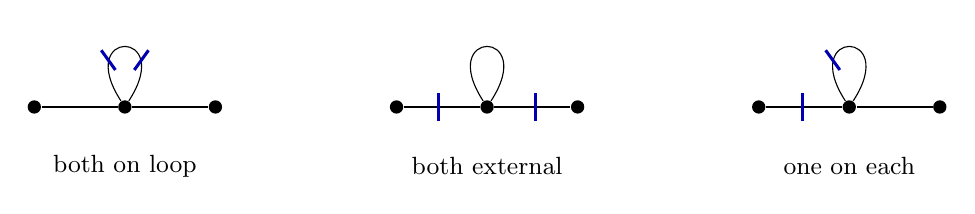
\begin{tikzpicture}[
   x=1cm,y=1cm,
   ext/.style={circle,fill=black,inner sep=1.7pt},
   dmark/.style={blue!70!black,line width=1.1pt},
   every node/.style={font=\small}
 ]
  \foreach \x/\i in {-4.6/1,0/2,4.6/3} {
    \node[ext] (l\i) at (\x-1.15,0) {};
    \node[ext] (r\i) at (\x+1.15,0) {};
    \node[ext] (v\i) at (\x,0) {};
    \draw (l\i)--(v\i)--(r\i);
    \draw (v\i) .. controls (\x-0.65,1.0) and (\x+0.65,1.0) .. (v\i);
  }
  \draw[dmark] (-4.9,0.72)--(-4.72,0.47);
  \draw[dmark] (-4.3,0.72)--(-4.48,0.47);
  \node at (-4.6,-0.75) {both on loop};

  \draw[dmark] (-0.62,-0.18)--(-0.62,0.18);
  \draw[dmark] (0.62,-0.18)--(0.62,0.18);
  \node at (0,-0.75) {both external};

  \draw[dmark] (4.0,-0.18)--(4.0,0.18);
  \draw[dmark] (4.3,0.72)--(4.48,0.47);
  \node at (4.6,-0.75) {one on each};
 \end{tikzpicture}
 \caption{Derivative-decorated one-vertex contractions. The loop-loop
 placement diverges, the external placement is finite, and a mixed placement
 gives an odd loop integral.}
 \label{fig:253a-derivative-topologies}
\end{figure}

% SOURCE-CONFLICT: Physical p. 57 suppresses derivative subscripts in its top contraction line. The proposal uses partial_{tau'} according to the p. 56 vertex and the reconciled equation index.
% YIN-SOURCE: id=PROPOSAL-B-U055; arguments=YIN253A-C02-A14; notes=253a:46; pdf=57; video=TtMNnZ8__UU:00:10:24.420-00:18:54.020; transcript=YIN253A-C02-T000769..YIN253A-C02-T000784; equations=YIN253A-C02-EQ021; class=SOURCE_COMPOSITE
For the first placement there are two ways to attach the undifferentiated
fields to the external insertions. The result is

% YIN-SOURCE: id=PROPOSAL-B-U056; arguments=YIN253A-C02-A14; notes=253a:46; pdf=57; video=TtMNnZ8__UU:00:10:24.420-00:18:54.020; transcript=YIN253A-C02-T000769..YIN253A-C02-T000784; equations=YIN253A-C02-EQ021; class=SOURCE_COMPOSITE
\begin{equation}
 \begin{aligned}
 2\cdot\frac{g}{8}\int d\tau'\,
 G_0(\tau-\tau')G_0(\tau')
 \langle\partial_{\tau'}\phi(\tau')
 \partial_{\tau'}\phi(\tau')\rangle_0
 &=\frac{g}{4}\int d\tau'\,
 G_0(\tau-\tau')G_0(\tau')[-\partial^2G_0(0)]\\
 &=\frac{g}{4}\int\frac{dk}{2\pi}
 \frac{e^{ik\tau}}{(k^2+1)^2}
 \int\frac{dk'}{2\pi}\frac{k'^2}{k'^2+1}.
 \end{aligned}
 \label{eq:253a-divergent-derivative-contraction}
\end{equation}

% YIN-SOURCE: id=PROPOSAL-B-U057; arguments=YIN253A-C02-A14; notes=253a:46; pdf=57; video=TtMNnZ8__UU:00:15:02.339-00:20:36.780; transcript=YIN253A-C02-T000778..YIN253A-C02-T000787; equations=YIN253A-C02-EQ021; class=SOURCE_COMPOSITE
We have a problem: this is divergent. Since $G_0(\tau)=\tfrac12e^{-|\tau|}$,
its second derivative is singular at coincidence. Equivalently, the loop
integrand tends to one as $|k'|\to\infty$. The calculation was completely
correct; it has exposed the short-distance content of the path-integral
measure.

% YIN-SOURCE: id=PROPOSAL-B-U058; arguments=YIN253A-C02-A14; notes=253a:46; pdf=57; video=TtMNnZ8__UU:00:18:55.500-00:20:36.780; transcript=YIN253A-C02-T000785..YIN253A-C02-T000787; equations=YIN253A-C02-EQ021; class=SOURCE_COMPOSITE
The other derivative placements are finite. When both derivatives act on the
external lines, the numerator is $k^2$; a mixed placement leaves an integrand
odd in the loop wave number:

% YIN-SOURCE: id=PROPOSAL-B-U059; arguments=YIN253A-C02-A14; notes=253a:46; pdf=57; video=TtMNnZ8__UU:00:18:08.840-00:20:36.780; transcript=YIN253A-C02-T000784..YIN253A-C02-T000787; equations=YIN253A-C02-EQ021; class=SOURCE_COMPOSITE
\begin{equation}
 \begin{aligned}
 &\frac{g}{4}\int\frac{dk}{2\pi}
 \frac{e^{ik\tau}k^2}{(k^2+1)^2}
 \int\frac{dk'}{2\pi}\frac{1}{k'^2+1},\\
 &\frac{g}{2}\int\frac{dk}{2\pi}
 \frac{e^{ik\tau}ik}{(k^2+1)^2}
 \int\frac{dk'}{2\pi}\frac{ik'}{k'^2+1}=0.
 \end{aligned}
 \label{eq:253a-finite-derivative-contractions}
\end{equation}

% YIN-SOURCE: id=PROPOSAL-B-U060; arguments=YIN253A-C02-A14; notes=253a:47; pdf=58; video=TtMNnZ8__UU:00:20:34.500-00:25:56.340; transcript=YIN253A-C02-T000788..YIN253A-C02-T000800; equations=YIN253A-C02-EQ021; class=SOURCE_COMPOSITE
The divergence comes from integrating modes with arbitrarily large wave
number. We therefore define the measure with a cutoff before performing any
Wick contraction:

% YIN-SOURCE: id=PROPOSAL-B-U061; arguments=YIN253A-C02-A14; notes=253a:47; pdf=58; video=TtMNnZ8__UU:00:21:28.919-00:25:13.980; transcript=YIN253A-C02-T000790..YIN253A-C02-T000798; equations=YIN253A-C02-EQ021; class=SOURCE_COMPOSITE
\begin{equation}
 [D\phi]=\prod_k d\widetilde\phi_k
 \quad\longrightarrow\quad
 [D\phi]_\Lambda=\prod_{|k|<\Lambda}d\widetilde\phi_k,
 \qquad
 G(\tau)=\int\frac{dk}{2\pi}
 \frac{e^{ik\tau}}{k^2+1-\Sigma(k)}.
 \label{eq:253a-cutoff-measure}
\end{equation}

\subsection{Counterterms and the definition of the path integral}
\label{sec:253a-counterterms}

% SOURCE-CONFLICT: In EQ022 the first loop integral carries |k'|<Lambda and the second has no visible cutoff subscript. The display below preserves this page-local distinction.
% YIN-SOURCE: id=PROPOSAL-B-U062; arguments=YIN253A-C02-A15; notes=253a:48; pdf=59; video=TtMNnZ8__UU:00:26:19.320-00:30:27.799; transcript=YIN253A-C02-T000802..YIN253A-C02-T000810; equations=YIN253A-C02-EQ022; class=SOURCE_COMPOSITE
With this regularization, the order-$g$ self-energy is a well-defined function
of $\Lambda$. The loop-loop derivative contraction supplies its linear
divergence, while the finite derivative placement supplies the $k^2$ term:

% YIN-SOURCE: id=PROPOSAL-B-U063; arguments=YIN253A-C02-A15; notes=253a:48; pdf=59; video=TtMNnZ8__UU:00:26:49.020-00:30:27.799; transcript=YIN253A-C02-T000803..YIN253A-C02-T000810; equations=YIN253A-C02-EQ022; class=SOURCE_COMPOSITE
\begin{equation}
 \begin{aligned}
 \Sigma(k)&=\frac{g}{4}\int_{|k'|<\Lambda}\frac{dk'}{2\pi}
 \frac{k'^2}{k'^2+1}
 +\frac{g}{4}k^2\int\frac{dk'}{2\pi}\frac{1}{k'^2+1}+O(g^2)\\
 &=\frac{g}{4}\left(\frac{k^2}{2}+\frac{\Lambda}{\pi}
 -\frac{1}{2}+O(\Lambda^{-1})\right)+O(g^2).
 \end{aligned}
 \label{eq:253a-cutoff-self-energy}
\end{equation}

% SOURCE-CONFLICT: Physical p. 59 qualifies the Hamiltonian as harmless at least for g<0 and leaves the operator ordering open. The proposal keeps the ordering issue in the quantization discussion without importing the source's unresolved punctuation.
% YIN-SOURCE: id=PROPOSAL-B-U064; arguments=YIN253A-C02-A15; notes=253a:48-49; pdf=59-60; video=TtMNnZ8__UU:00:30:29.880-00:35:38.839; transcript=YIN253A-C02-T000811..YIN253A-C02-T000821; equations=YIN253A-C02-EQ022; class=SOURCE_COMPOSITE
To identify the quantum order of this effect, we restore $\hbar$. The Gaussian
propagator carries one power of $\hbar$, and every interaction vertex from the
expansion of the Euclidean weight carries $1/\hbar$:

% SOURCE-CONFLICT: Physical p. 60 writes a questioned +O(hbar) correction in L^E. The proposal places the definite correction in Delta L^E below and withholds the question mark from reader-facing mathematics.
% YIN-SOURCE: id=PROPOSAL-B-U065; arguments=YIN253A-C02-A15; notes=253a:48-49; pdf=59-60; video=TtMNnZ8__UU:00:30:44.340-00:37:15.720; transcript=YIN253A-C02-T000812..YIN253A-C02-T000826; equations=YIN253A-C02-EQ022; class=SOURCE_COMPOSITE
\begin{equation}
 \begin{aligned}
 Z&=\int[Dq]\exp\left[-\frac{1}{\hbar}\int d\tau\,L^E\right],\\
 L^E_{\mathrm{cl}}&=\frac{1}{2}(\partial_\tau q)^2+\frac{1}{2}q^2
 -\frac{g}{8}q^2(\partial_\tau q)^2,\\
 \widetilde G(k)&=\frac{\hbar}{k^2+1-\Sigma(k)},\\
 \Sigma(k)&=\frac{\hbar g}{4}
 \left(\frac{k^2}{2}+\frac{\Lambda}{\pi}-\frac{1}{2}
 +O(\Lambda^{-1})\right)+O(\hbar^2g^2).
 \end{aligned}
 \label{eq:253a-restored-hbar}
\end{equation}

% YIN-SOURCE: id=PROPOSAL-B-U066; arguments=YIN253A-C02-A15; notes=253a:49; pdf=60; video=TtMNnZ8__UU:00:31:33.840-00:39:39.780; transcript=YIN253A-C02-T000814..YIN253A-C02-T000830; equations=YIN253A-C02-EQ022; class=SOURCE_COMPOSITE
The classical expression fixes the $\hbar\to0$ limit. Quantum mechanics also
permits local terms of order $\hbar$, arising from the ordering prescription
or from the Jacobian of a nonlinear coordinate change. We choose a quadratic
counterterm that corrects the oscillator frequency:

% YIN-SOURCE: id=PROPOSAL-B-U067; arguments=YIN253A-C02-A15; notes=253a:49; pdf=60; video=TtMNnZ8__UU:00:37:57.300-00:40:01.820; transcript=YIN253A-C02-T000828..YIN253A-C02-T000831; equations=YIN253A-C02-EQ022; class=SOURCE_COMPOSITE
\begin{equation}
 \Delta L^E=c\,g\hbar\frac{q^2}{2}.
 \label{eq:253a-quadratic-counterterm}
\end{equation}

% YIN-SOURCE: id=PROPOSAL-B-U068; arguments=YIN253A-C02-A15; notes=253a:49; pdf=60; video=TtMNnZ8__UU:00:40:02.280-00:43:36.060; transcript=YIN253A-C02-T000832..YIN253A-C02-T000837; equations=YIN253A-C02-EQ022; class=SOURCE_COMPOSITE
This term shifts the self-energy by $-cg\hbar$. Including it gives

% SOURCE-CONFLICT: Physical p. 60 uses O(hbar^2 g^2) before the counterterm and O(g^2) afterward. Both source-local orders are retained in their respective displays.
% YIN-SOURCE: id=PROPOSAL-B-U069; arguments=YIN253A-C02-A15; notes=253a:49; pdf=60; video=TtMNnZ8__UU:00:40:50.720-00:43:36.060; transcript=YIN253A-C02-T000833..YIN253A-C02-T000837; equations=YIN253A-C02-EQ022; class=SOURCE_COMPOSITE
\begin{equation}
 \Sigma(k)=\hbar g\left(
 \frac{k^2}{8}+\frac{\Lambda}{4\pi}-\frac{1}{8}-c
 +O(\Lambda^{-1})\right)+O(g^2).
 \label{eq:253a-counterterm-self-energy}
\end{equation}

% YIN-SOURCE: id=PROPOSAL-B-U070; arguments=YIN253A-C02-A15; notes=253a:50; pdf=61; video=TtMNnZ8__UU:00:43:31.260-00:45:38.819; transcript=YIN253A-C02-T000838..YIN253A-C02-T000841; equations=YIN253A-C02-EQ023; class=SOURCE_COMPOSITE
Choosing

% YIN-SOURCE: id=PROPOSAL-B-U071; arguments=YIN253A-C02-A15; notes=253a:50; pdf=61; video=TtMNnZ8__UU:00:43:31.260-00:44:39.240; transcript=YIN253A-C02-T000838..YIN253A-C02-T000839; equations=YIN253A-C02-EQ023; class=SOURCE_COMPOSITE
\begin{equation}
 c=\frac{\Lambda}{4\pi}+c_{\mathrm{fin}}
 \label{eq:253a-counterterm-choice}
\end{equation}

% YIN-SOURCE: id=PROPOSAL-B-U072; arguments=YIN253A-C02-A15; notes=253a:50; pdf=61; video=TtMNnZ8__UU:00:43:31.260-00:46:09.900; transcript=YIN253A-C02-T000838..YIN253A-C02-T000842; equations=YIN253A-C02-EQ023; class=SOURCE_COMPOSITE
makes the $\Lambda\to\infty$ limit finite. The divergent part of $c$ is fixed
by this requirement. Its finite part specifies which quantization of the
classical expression has been chosen. Of the counterterm, that finite part is
physics: it must be fixed by additional input.

% SOURCE-CONFLICT: Physical pp. 61-62 call the gap unambiguous while leaving the finite part of c undetermined. The proposal states the reconciled claim: the gap is physical after the finite quantization input has been fixed.
% YIN-SOURCE: id=PROPOSAL-B-U073; arguments=YIN253A-C02-A15; notes=253a:50-51; pdf=61-62; video=TtMNnZ8__UU:00:43:31.260-00:48:59.599; transcript=YIN253A-C02-T000838..YIN253A-C02-T000847; equations=YIN253A-C02-EQ023; class=SOURCE_COMPOSITE
Once that finite input is fixed, the pole of the regulated propagator has a
finite limit and yields the physical energy gap:

% YIN-SOURCE: id=PROPOSAL-B-U074; arguments=YIN253A-C02-A15; notes=253a:50-51; pdf=61-62; video=TtMNnZ8__UU:00:43:31.260-00:48:59.599; transcript=YIN253A-C02-T000838..YIN253A-C02-T000847; equations=YIN253A-C02-EQ023; class=SOURCE_COMPOSITE
\begin{equation}
 \begin{aligned}
 \widetilde G(k)&=\frac{\hbar}{k^2+1-\Sigma(k)}
 \quad\text{has a pole at }k=i\omega_1,\\
 \omega_1&=1+\hbar g\left(-\frac{\Lambda}{8\pi}
 +\frac{c}{2}+\frac{1}{8}\right)+O(g^2)
 =\widehat E_1-\widehat E_0.
 \end{aligned}
 \label{eq:253a-renormalized-gap}
\end{equation}

% YIN-SOURCE: id=PROPOSAL-B-U075; arguments=YIN253A-C02-A15; notes=253a:51; pdf=62; video=TtMNnZ8__UU:00:45:00.540-00:50:10.099; transcript=YIN253A-C02-T000841..YIN253A-C02-T000849; equations=YIN253A-C02-EQ023; class=SOURCE_COMPOSITE
The regularization scheme and its counterterms belong to the definition of the
path integral. Ordinary quantum mechanics allows broad freedom in specifying
the Hamiltonian. In QFT, Poincar\'e symmetry and causality sharply restrict the
counterterms and fix them up to a small ambiguity.

% PROPOSED-EDITORIAL-BOUNDARY: Problem Set 2 occupies physical pp. 63-67 and remains deferred to the assignment-integration pass; no problem statement, diagram, or formula from those pages is imported here. Physical p. 68 is used only as the Chapter 3 boundary.
% PROPOSAL-B-INVENTORY: arguments=YIN253A-C02-A09,YIN253A-C02-A10,YIN253A-C02-A11,YIN253A-C02-A12,YIN253A-C02-A13,YIN253A-C02-A14,YIN253A-C02-A15.
% PROPOSAL-B-INVENTORY: equations=YIN253A-C02-EQ013-EQ014 quartic expansion and first graphs; YIN253A-C02-EQ015-EQ016 connected exponentiation and E_0; YIN253A-C02-EQ017-EQ018 normalized two-point function and self-energy; YIN253A-C02-EQ019 dressed poles and gap; YIN253A-C02-EQ020-EQ021 coordinate redefinition, derivative vertex, divergence, and cutoff; YIN253A-C02-EQ022-EQ023 restored hbar, counterterm, finite part, and physical pole.
% PROPOSAL-B-INVENTORY: notes=253a:30,31,32,33,34,35,36,37,38,39,40,41,42,43,44,45,46,47,48,49,50,51; pdf=41-62.
% PROPOSAL-B-INVENTORY: voice-cues-used=VOICE-0068 undergraduate-QM check; VOICE-0073 asymptotic feature; VOICE-0075 exponentiation follows from expansion; VOICE-0079 one extensive connected divergence; VOICE-0082 graphs organize contractions; VOICE-0084 four-times-three count; VOICE-0085 counting emphasis; VOICE-0087 return to formula; VOICE-0089 1PI question; VOICE-0091 Fourier representation looks weird; VOICE-0095 finite-order meaning; VOICE-0097 coordinate freedom; VOICE-0101 divergent problem; VOICE-0103 calculation correct; VOICE-0110 order-hbar freedom lightly recast; VOICE-0117 finite counterterm is physics; VOICE-0124 Poincare and causality restriction lightly recast.
% PROPOSAL-B-INVENTORY: source-conflicts-withheld=quartic phi-versus-q; G-versus-G_0 reminder; x-versus-q endpoint labels; unlabeled Im-k axis and lower poles; O(g^3)-versus-continuation-dots; open operator-ordering annotation; derivative-subscript omissions; discrete coefficient-measure notation; missing cutoff label on the second EQ022 integral; questioned O(hbar) correction; O(hbar^2g^2)-versus-O(g^2) remainders; finite-c ambiguity versus the physical-gap statement; Problem-Set-2 and Chapter-3 boundary material.
